\documentclass[a4paper,10pt]{book}
\usepackage[utf8]{inputenc}
\usepackage{fullpage}
\usepackage{cite}
\usepackage[utf8]{inputenc}
\usepackage{a4wide}
\usepackage{url}
\usepackage{graphicx}
\usepackage{caption}
\usepackage{float} % para que los gr\'aficos se queden en su lugar con [H]
\usepackage{subcaption}
\usepackage{wrapfig}
\usepackage{color}
\usepackage{amsmath} %para escribir funci\'on partida , matrices
\usepackage{amsthm} %para numerar definciones y teoremas
\usepackage[hidelinks]{hyperref} % para inlcuir links dentro del texto
\usepackage{tabu} 
\usepackage{comment}
\usepackage{amsfonts} % \mathbb{N} -> conjunto de los n\'umeros naturales  
\usepackage{enumerate}
\usepackage{listings}
\usepackage[colorinlistoftodos, textsize=small]{todonotes} % Para poner notas en el medio del texto!! No olvidar hacer. 
\usepackage{framed} % Para encuadrar texto. \begin{framed}
\usepackage{csquotes} % Para citar texto \begin{displayquote}
\usepackage{epigraph} % Epigrafe  \epigraph{texto}{\textit{autor}}
\usepackage{authblk}
\usepackage{titlesec}
\usepackage{varioref}
\usepackage{bm} % \bm{\alpha} bold greek symbol
\usepackage{pdfpages} % \includepdf
\usepackage[makeroom]{cancel} % \cancel{} \bcancel{} etc
\usepackage{wrapfig} % \begin{wrapfigure} Pone figura al lado del texto
\usepackage{mdframed}
\usepackage{algorithm}
%\usepackage{quoting}
\usepackage{mathtools}	
\usepackage{tikz}
\usepackage{paracol}

\newcommand{\vm}[1]{\mathbf{#1}}
\newcommand{\N}{\mathcal{N}}
\newcommand{\citel}[1]{\cite{#1}\label{#1}}
\newcommand\hfrac[2]{\genfrac{}{}{0pt}{}{#1}{#2}} %\frac{}{} sin la linea del medio

\newtheorem{midef}{Definition}
\newtheorem{miteo}{Theorem}
\newtheorem{mipropo}{Proposition}

\theoremstyle{definition}
\newtheorem{definition}{Definition}[section]
\newtheorem{theorem}{Theorem}[section]
\newtheorem{proposition}{Proposition}[section]


%http://latexcolor.com/
\definecolor{azul}{rgb}{0.36, 0.54, 0.66}
\definecolor{rojo}{rgb}{0.7, 0.2, 0.116}
\definecolor{rojopiso}{rgb}{0.8, 0.25, 0.17}
\definecolor{verdeingles}{rgb}{0.12, 0.5, 0.17}
\definecolor{ubuntu}{rgb}{0.44, 0.16, 0.39}
\definecolor{debian}{rgb}{0.84, 0.04, 0.33}
\definecolor{dkgreen}{rgb}{0,0.6,0}
\definecolor{gray}{rgb}{0.5,0.5,0.5}
\definecolor{mauve}{rgb}{0.58,0,0.82}

\lstset{
  language=Python,
  aboveskip=3mm,
  belowskip=3mm,
  showstringspaces=true,
  columns=flexible,
  basicstyle={\small\ttfamily},
  numbers=none,
  numberstyle=\tiny\color{gray},
  keywordstyle=\color{blue},
  commentstyle=\color{dkgreen},
  stringstyle=\color{mauve},
  breaklines=true,
  breakatwhitespace=true,
  tabsize=4
}

% tikzlibrary.code.tex
%
% Copyright 2010-2011 by Laura Dietz
% Copyright 2012 by Jaakko Luttinen
%
% This file may be distributed and/or modified
%
% 1. under the LaTeX Project Public License and/or
% 2. under the GNU General Public License.
%
% See the files LICENSE_LPPL and LICENSE_GPL for more details.

% Load other libraries

%\newcommand{\vast}{\bBigg@{2.5}}
% newcommand{\Vast}{\bBigg@{14.5}}
% \usepackage{helvet}
% \renewcommand{\familydefault}{\sfdefault}

\usetikzlibrary{shapes}
\usetikzlibrary{fit}
\usetikzlibrary{chains}
\usetikzlibrary{arrows}

% Latent node
\tikzstyle{latent} = [circle,fill=white,draw=black,inner sep=1pt,
minimum size=20pt, font=\fontsize{10}{10}\selectfont, node distance=1]
% Observed node
\tikzstyle{obs} = [latent,fill=gray!25]
% Invisible node
\tikzstyle{invisible} = [latent,minimum size=0pt,color=white, opacity=0, node distance=0]
% Constant node
\tikzstyle{const} = [rectangle, inner sep=0pt, node distance=0.1]
%state
\tikzstyle{estado} = [latent,minimum size=8pt,node distance=0.4]
%action
\tikzstyle{accion} =[latent,circle,minimum size=5pt,fill=black,node distance=0.4]
\tikzstyle{fijo} =[latent,circle,minimum size=5pt,fill=black]


% Factor node
\tikzstyle{factor} = [rectangle, fill=black,minimum size=10pt, draw=black, inner
sep=0pt, node distance=1]
% Deterministic node
\tikzstyle{det} = [latent, rectangle]

% Plate node
\tikzstyle{plate} = [draw, rectangle, rounded corners, fit=#1]
% Invisible wrapper node
\tikzstyle{wrap} = [inner sep=0pt, fit=#1]
% Gate
\tikzstyle{gate} = [draw, rectangle, dashed, fit=#1]

% Caption node
\tikzstyle{caption} = [font=\footnotesize, node distance=0] %
\tikzstyle{plate caption} = [caption, node distance=0, inner sep=0pt,
below left=5pt and 0pt of #1.south east] %
\tikzstyle{factor caption} = [caption] %
\tikzstyle{every label} += [caption] %

\tikzset{>={triangle 45}}

%\pgfdeclarelayer{b}
%\pgfdeclarelayer{f}
%\pgfsetlayers{b,main,f}

% \factoredge [options] {inputs} {factors} {outputs}
\newcommand{\factoredge}[4][]{ %
  % Connect all nodes #2 to all nodes #4 via all factors #3.
  \foreach \f in {#3} { %
    \foreach \x in {#2} { %
      \path (\x) edge[-,#1] (\f) ; %
      %\draw[-,#1] (\x) edge[-] (\f) ; %
    } ;
    \foreach \y in {#4} { %
      \path (\f) edge[->,#1] (\y) ; %
      %\draw[->,#1] (\f) -- (\y) ; %
    } ;
  } ;
}

% \edge [options] {inputs} {outputs}
\newcommand{\edge}[3][]{ %
  % Connect all nodes #2 to all nodes #3.
  \foreach \x in {#2} { %
    \foreach \y in {#3} { %
      \path (\x) edge [->,#1] (\y) ;%
      %\draw[->,#1] (\x) -- (\y) ;%
    } ;
  } ;
}

% \factor [options] {name} {caption} {inputs} {outputs}
\newcommand{\factor}[5][]{ %
  % Draw the factor node. Use alias to allow empty names.
  \node[factor, label={[name=#2-caption]#3}, name=#2, #1,
  alias=#2-alias] {} ; %
  % Connect all inputs to outputs via this factor
  \factoredge {#4} {#2-alias} {#5} ; %
}

% \plate [options] {name} {fitlist} {caption}
\newcommand{\plate}[4][]{ %
  \node[wrap=#3] (#2-wrap) {}; %
  \node[plate caption=#2-wrap] (#2-caption) {#4}; %
  \node[plate=(#2-wrap)(#2-caption), #1] (#2) {}; %
}

% \gate [options] {name} {fitlist} {inputs}
\newcommand{\gate}[4][]{ %
  \node[gate=#3, name=#2, #1, alias=#2-alias] {}; %
  \foreach \x in {#4} { %
    \draw [-*,thick] (\x) -- (#2-alias); %
  } ;%
}

% \vgate {name} {fitlist-left} {caption-left} {fitlist-right}
% {caption-right} {inputs}
\newcommand{\vgate}[6]{ %
  % Wrap the left and right parts
  \node[wrap=#2] (#1-left) {}; %
  \node[wrap=#4] (#1-right) {}; %
  % Draw the gate
  \node[gate=(#1-left)(#1-right)] (#1) {}; %
  % Add captions
  \node[caption, below left=of #1.north ] (#1-left-caption)
  {#3}; %
  \node[caption, below right=of #1.north ] (#1-right-caption)
  {#5}; %
  % Draw middle separation
  \draw [-, dashed] (#1.north) -- (#1.south); %
  % Draw inputs
  \foreach \x in {#6} { %
    \draw [-*,thick] (\x) -- (#1); %
  } ;%
}

% \hgate {name} {fitlist-top} {caption-top} {fitlist-bottom}
% {caption-bottom} {inputs}
\newcommand{\hgate}[6]{ %
  % Wrap the left and right parts
  \node[wrap=#2] (#1-top) {}; %
  \node[wrap=#4] (#1-bottom) {}; %
  % Draw the gate
  \node[gate=(#1-top)(#1-bottom)] (#1) {}; %
  % Add captions
  \node[caption, above right=of #1.west ] (#1-top-caption)
  {#3}; %
  \node[caption, below right=of #1.west ] (#1-bottom-caption)
  {#5}; %
  % Draw middle separation
  \draw [-, dashed] (#1.west) -- (#1.east); %
  % Draw inputs
  \foreach \x in {#6} { %
    \draw [-*,thick] (\x) -- (#1); %
  } ;%
}


\usepackage{physics}
\newcommand*\diff{\mathop{}\!\mathrm{d}}

\newif\ifen
\newif\ifes
\newcommand{\en}[1]{\ifen#1\fi}
\newcommand{\es}[1]{\ifes#1\fi}
\estrue


%opening
\title{\huge Habilidad y evolución cultural}
\author{Gustavo Landfried}

\begin{document}

\maketitle

\tableofcontents

\chapter*{Abstract}


\chapter{Conocimiento empírico}

\epigraph{El conocimiento empírico no es más que principio de incertidumbre compatible con la evidencia formal y empíricia}{}

\section{Creencias}

La ciencia es una institución humana que tiene pretención de verdad, esto es de formular proposiciones que valgan para todas las personas, tanto intercultural como intersubjetivamente.
Las ciencias formales validan sus proposiciones mediante teoremas, resultados derivados de aplicar las reglas internas a un sistema axiomático cerrado.
% Las ciencias de la computación nacen como una rama de las matemáticas aplicadas, y desarrolla en el transcurso de su historia orientaciones tanto de ciencias formales (algoritmos, lógica y computabilidad) y como de ciencias empíricas (simulación, inteligencia artificial).
% A diferencia de las ciencia formales, 
Las ciencias empíricas deben validar sus proposiciones dentro de sistemas abiertos, lo que impone siempre un grado de incertidumbre asociada.
¿Cuál es entonces la fuente de validez del conocimiento empírico?


\subsection{Principio de incertidumbre}

Supongamos que tenemos 3 cajas y sabemos que detrás de una hay un regalo.
Una posible distribuión de creencias es:

\begin{figure}[H]
\centering
\tikz{ %
        
         \node[factor, minimum size=1cm] (p1) {} ;
         \node[factor, minimum size=1cm, xshift=1.5cm] (p2) {} ;
         \node[factor, minimum size=1cm, xshift=3cm] (p3) {} ;
         \node[const, above=of p1, yshift=.15cm] (fp1) {$1/10$};
         \node[const, above=of p2, yshift=.15cm] (fp2) {$8/10$};
         \node[const, above=of p3, yshift=.15cm] (fp3) {$1/10$};
        } 
\end{figure}

lo que representa una preferencia parcial por la caja del medio.
Pero si de verdad no tenemos ninguna información respecto de dónde está el regalo, no hay motivos para tener preferencia por ninguna de las opciones, lo que sin lugar a dudas nos hará estar de acuerdo en la siguiente distribución de creencias.

\begin{figure}[H]
\centering
\tikz{ %
        
         \node[factor, minimum size=1cm] (p1) {} ;
         \node[factor, minimum size=1cm, xshift=1.5cm] (p2) {} ;
         \node[factor, minimum size=1cm, xshift=3cm] (p3) {} ;
         \node[const, above=of p1, yshift=.15cm] (fp1) {$1/3$};
         \node[const, above=of p2, yshift=.15cm] (fp2) {$1/3$};
         \node[const, above=of p3, yshift=.15cm] (fp3) {$1/3$};
        } 
\end{figure}

Este tipo de distribuciones de creencias, que permiten el acuerdo intersubjetivo, la vamos a llamar \textbf{creencia honesta}.
Las creencias honestas son las que maximizan incertidumbre, siendo coherente con la información disponible.
En este caso, en el que no tenemos información previa, la obtuvimos dividiendo la creencia en partes iguales.
Éste es un viejo principio conocido como ``de indiferencia''.
¿Pero cómo hacemos para actualizar las creencias de forma honesta cuando recibimos nueva información?

\begin{figure}[H]
\centering
\tikz{ %
         \node[factor, minimum size=1cm] (p1) {} ;
         \node[det, minimum size=1cm, xshift=1.5cm] (p2) {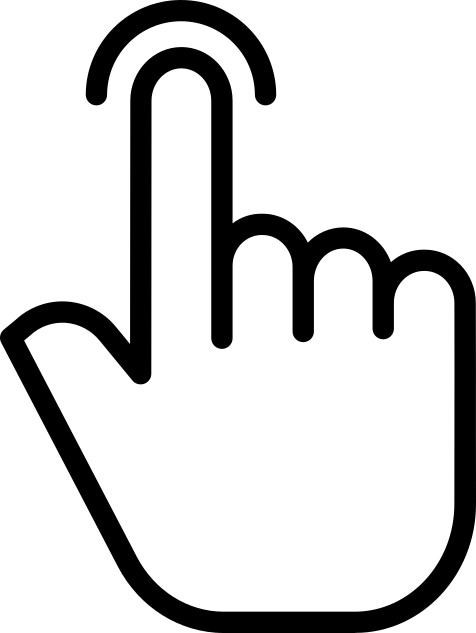
\includegraphics[width=0.03\textwidth]{static/dedo.png}} ;
         \node[factor, minimum size=1cm, xshift=3cm] (p3) {} ;

         \node[const, above=of p1, yshift=.15cm] (fp1) {$?$};
         \node[const, above=of p2, yshift=.15cm] (fp2) {$0$};
         \node[const, above=of p3, yshift=.15cm] (fp3) {$?$};
         \node[const, below=of p2, yshift=-.10cm, xshift=0.3cm] (dedo) {};
        } 
\end{figure}

Aquí recibimos el dato de que el regalo no está en la caja del medio, lo que nos permite asignar creencia 0 a esa caja.
Para actualizar el resto de las cajas necesitamos interpretar qué nos está diciendo la pista.
Supongamos que la pista depende de dónde está el regalo, sólo nos puede indicar dónde no está el regalo.
Esto lo podemos representar con el siguiente modelo causal.

\begin{figure}[H]
\centering
\tikz{            
    \node[latent,] (r) {
\includegraphics[width=0.06\textwidth]{static/regalo.png}} ;
    \node[const,left=of r] (nr) {\Large $r$} ;    
    
    
    \node[latent, below=of r] (d) {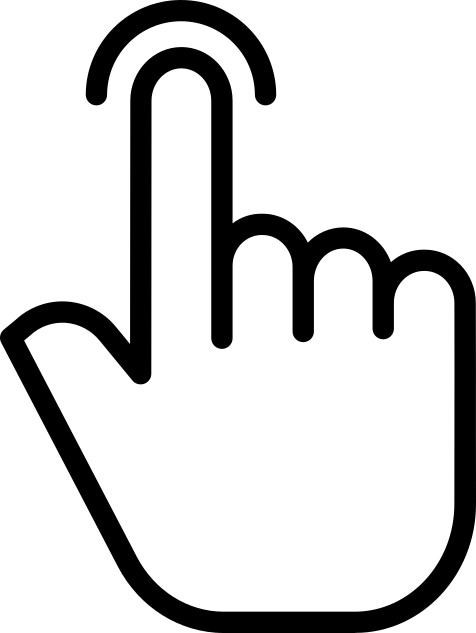
\includegraphics[width=0.05\textwidth]{static/dedo.png}} ;
    \node[const, left=of d] (nd) {\Large $s$} ;

    \edge {r} {d};
            
}
\end{figure}

Siguiendo con el principio de indiferencia que usamos para definir una creencia honesta, dividimos la creencia en partes iguales por los caminos del modelo causal para definir la creencia honesta de ellos.

\begin{figure}[H]
\centering
\tikz{
\node[latent, draw=white, yshift=0.6cm] (b0) {$ 1$};

\node[latent,below=of b0,yshift=0.6cm, xshift=-3cm] (r1) {$r_1$};
\node[latent,below=of b0,yshift=0.6cm] (r2) {$r_2$};
\node[latent,below=of b0,yshift=0.6cm, xshift=3cm] (r3) {$r_3$};

\node[latent, below=of r1, draw=white, yshift=0.6cm] (br1) {$\frac{1}{3}$};
\node[latent, below=of r2, draw=white, yshift=0.6cm] (br2) {$\frac{1}{3}$};
\node[latent, below=of r3, draw=white, yshift=0.6cm] (br3) {$\frac{1}{3}$};
\node[latent,below=of br1,yshift=0.6cm, xshift=-0.7cm] (r1d2) {$s_2$};
\node[latent,below=of br1,yshift=0.6cm, xshift=0.7cm] (r1d3) {$s_3$};

\node[latent,below=of r1d2,yshift=0.6cm,draw=white] (br1d2) {$\frac{1}{3}\frac{1}{2}$};
\node[latent,below=of r1d3,yshift=0.6cm, draw=white] (br1d3) {$\frac{1}{3}\frac{1}{2}$};
\node[latent,below=of br2,yshift=0.6cm, xshift=-0.7cm] (r2d1) {$s_1$};
\node[latent,below=of br2,yshift=0.6cm, xshift=0.7cm] (r2d3) {$s_3$};
\node[latent,below=of br3,yshift=0.6cm, xshift=-0.7cm] (r3d1) {$s_1$};
\node[latent,below=of br3,yshift=0.6cm, xshift=0.7cm] (r3d2) {$s_2$};

\node[latent,below=of r2d1,yshift=0.6cm, draw=white] (br2d1) {$\frac{1}{3}\frac{1}{2}$};
\node[latent,below=of r2d3,yshift=0.6cm,draw=white] (br2d3) {$\frac{1}{3}\frac{1}{2}$};
\node[latent,below=of r3d1,yshift=0.6cm, draw=white] (br3d1) {$\frac{1}{3}\frac{1}{2}$};
\node[latent,below=of r3d2,yshift=0.6cm,draw=white] (br3d2) {$\frac{1}{3}\frac{1}{2}$};
\edge[-] {b0} {r1,r2,r3};
\edge[-] {r1} {br1};
\edge[-] {r2} {br2};
\edge[-] {r3} {br3};
\edge[-] {br1} {r1d2,r1d3};
\edge[-] {r1d2} {br1d2};
\edge[-] {r1d3} {br1d3};
\edge[-] {br2} {r2d1, r2d3};
\edge[-] {br3} {r3d1,r3d2};
\edge[-] {r2d1} {br2d1};
\edge[-] {r2d3} {br2d3};
\edge[-] {r3d1} {br3d1};
\edge[-] {r3d2} {br3d2};
}
\end{figure}

Primero dividimos la creencia sobre el regalo en partes iguales, y luego volvemos a dividir la creencia sobre la pista en partes iguales.
Nuestra creencia conjunta honesta a priori es,

\begin{table}[H]
\centering
 \begin{tabular}{c|c|c|c|} \setlength\tabcolsep{0.4cm} 
        & \, $r_1$ \, &  \, $r_2$ \, & \, $r_3$ \, \\ \hline 
  $s_1$ & $0$ & $1/6$ & $1/6$  \\ \hline
  $s_2$ & $1/6$ & $0$ & $1/6$  \\ \hline
  $s_3$ & $1/6$ & $1/6$ & $0$ \\ \hline 
  \end{tabular}
\end{table}
  
Es honesta porque maximiza la incertidumbre dada la información disponible hasta el momento: el modelo causal.
Y es conjunta porque es la creencia de que ocurran simultaneamente ambas variables, $\text{Creencia}(r,s)$.

\subsection{Reglas de la probabilidad}

Las reglas de la probabilidad han sido derivadas formalmente a partir de una gran cantidad de sistemas axiomáticos conceptualmente distintos e independientes entre si, lo cual es uno de los punto fuertes a su favor.
Pero quizás más importante es que ellas garantizan maximizar la incertidumbre dada la información empírica (datos) y formal (modelos causales).

La teoría de la probabilidad tiene sólo dos reglas: la regla de la suma y la regla del producto.
La primera computa la creencia de una variable integrando en partes iguales la creencia conjunta.
Por ejemplo, la creencia honesta sobre los regalos nuevamente es 1/3
\begin{equation}
\text{Creencia}(r_i) = \sum_j \text{Creencia}(r_i, s_j) = 1/3
\end{equation}

y sobre la pista también
\begin{equation}
\text{Creencia}(s_j) = \sum_i \text{Creencia}(r_i, s_j) = 1/3
\end{equation}

La segunda regla consiste en quedarnos con la creencia a priori que es compatible con el dato, $\text{Creencia}(r_i, s_2)$.
%
\begin{table}[H]
\centering
 \begin{tabular}{c|c|c|c|c} \setlength\tabcolsep{0.4cm} 
        & \, $r_1$ \, &  \, $r_2$ \, & \, $r_3$ \, & \\ \hline 
  $s_1$ &  &  & & \\ \hline
  $s_2$ & $1/6$ & $0$ & $1/6$ & $1/3$ \\ \hline
  $s_3$ &  &  &  & \\ \hline 
  \end{tabular}
\end{table}
%
Lo que nos permitirá cumplir el objetivo que nos habíamos propuesto, actualizar la creencia sobre el regalo luego de haber visto la pista.
Como \textbf{la creencia que sobrevive} es ahora nuestra nueva creencia total, la normalizamos (en partes iguales) para que vuelva a sumar 1
%
\begin{equation}
\text{Creencia}(r_i| s_2) = \frac{\text{Creencia}(r_i, s_2)}{\text{Creencia}(s_2)} = 1/2
\end{equation}
%
La concusión a la que llegamos coincide con la intuición de la mayoría.
\begin{figure}[H]
\centering
\tikz{ %
        
         \node[factor, minimum size=1cm] (p1) {} ;
         \node[det, minimum size=1cm, xshift=1.5cm] (p2) {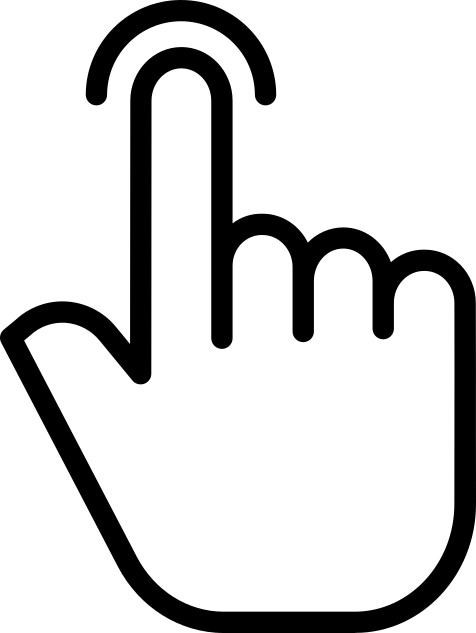
\includegraphics[width=0.03\textwidth]{static/dedo.png}} ;
         \node[factor, minimum size=1cm, xshift=3cm] (p3) {} ;

         \node[const, above=of p1, yshift=.15cm] (fp1) {$1/2$};
         \node[const, above=of p2, yshift=.15cm] (fp2) {$0$};
         \node[const, above=of p3, yshift=.15cm] (fp3) {$1/2$};
         \node[const, below=of p2, yshift=-.10cm, xshift=0.3cm] (dedo) {};
}
\end{figure}
%
Pero este resultado depende del modelo causal elegido.

\subsection{Modelos causales alternativos}

Supongamos que la pista, además de no poder coincidir con la posición del regalo, tiene prohibida una de las puertas.
Esto lo podemos representar con el siguiente modelo causal.

\begin{figure}[H]
\centering
\tikz{        
    
    \node[latent] (d) {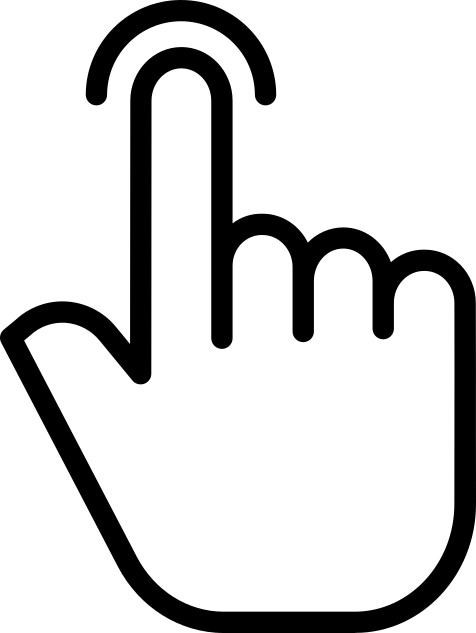
\includegraphics[width=0.05\textwidth]{static/dedo.png}} ;
    \node[const,above=of d] (nd) {\Large $s$} ;
    
    \node[latent, above=of d, xshift=-1.5cm] (r) {
\includegraphics[width=0.06\textwidth]{static/regalo.png}} ;
    \node[const,above=of r] (nr) {\Large $r$} ;
    
    \node[latent, fill=black!30, above=of d, xshift=1.5cm] (c) {
\includegraphics[width=0.06\textwidth]{static/cerradura.png}} ;
    \node[const,above=of c] (nc) {\Large $c=1$} ;
    
    \edge {r,c} {d};
}
\end{figure}

Este modelo es más conocido como el Monty Hall.
Para simplificar el problema, suponemos que la puerta 1 es la que queda cerrada, $c=1$.
Supongamos que en este contexto recibimos una pista.
%
\begin{figure}[H]
\centering
\tikz{ %
        
         \node[factor, minimum size=1cm] (p1) {
\includegraphics[width=0.025\textwidth]{static/cerradura.png}} ;
         \node[det, minimum size=1cm, xshift=1.5cm] (p2) {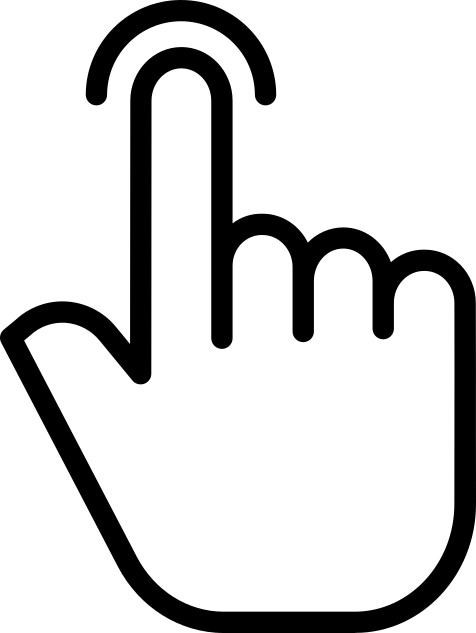
\includegraphics[width=0.03\textwidth]{static/dedo.png}} ;
         \node[factor, minimum size=1cm, xshift=3cm] (p3) {} ;
         \node[const, above=of p1, yshift=.15cm] (fp1) {$?$};
         \node[const, above=of p2, yshift=.15cm] (fp2) {$0$};
         \node[const, above=of p3, yshift=.15cm] (fp3) {$?$};
         \node[const, below=of p2, yshift=-.10cm, xshift=0.3cm] (dedo) {};
        
        } 
\end{figure}

¿Cómo hacemos para actualizar las creencias de forma honesta?
Como hicimos antes, maximizamos la incertidumbre dividiendo las creencias por los caminos del modelo causal de modo de definir la creencia conjunta honesta.

\begin{figure}[H]
\centering
\tikz{
\node[latent, draw=white, yshift=0.8cm] (b0) {$1$};
\node[latent,below=of b0,yshift=0.8cm, xshift=-2cm] (r1) {$r_1$};
\node[latent,below=of b0,yshift=0.8cm] (r2) {$r_2$};
\node[latent,below=of b0,yshift=0.8cm, xshift=2cm] (r3) {$r_3$};

\node[latent, below=of r1, draw=white, yshift=0.8cm] (br1) {$\frac{1}{3}$};
\node[latent, below=of r2, draw=white, yshift=0.8cm] (br2) {$\frac{1}{3}$};
\node[latent, below=of r3, draw=white, yshift=0.8cm] (br3) {$\frac{1}{3}$};
\node[latent,below=of br1,yshift=0.8cm] (c11) {$c_1$};
\node[latent,below=of br2,yshift=0.8cm] (c12) {$c_1$};
\node[latent,below=of br3,yshift=0.8cm] (c13) {$c_1$};

\node[latent, below=of c11, draw=white, yshift=0.8cm] (bc11) {$\frac{1}{3}$};
\node[latent, below=of c12, draw=white, yshift=0.8cm] (bc12) {$\frac{1}{3}$};
\node[latent, below=of c13, draw=white, yshift=0.8cm] (bc13) {$\frac{1}{3}$};
\node[latent,below=of bc11,yshift=0.8cm, xshift=-0.7cm] (r1d2) {$s_2$};
\node[latent,below=of bc11,yshift=0.8cm, xshift=0.7cm] (r1d3) {$s_3$};
\node[latent,below=of bc12,yshift=0.8cm] (r2d3) {$s_3$};
\node[latent,below=of bc13,yshift=0.8cm] (r3d2) {$s_2$};

\node[latent,below=of r1d2,yshift=0.8cm,draw=white] (br1d2) {$\frac{1}{3}\frac{1}{2}$};
\node[latent,below=of r1d3,yshift=0.8cm, draw=white] (br1d3) {$\frac{1}{3}\frac{1}{2}$};
\node[latent,below=of r2d3,yshift=0.8cm,draw=white] (br2d3) {$\frac{1}{3}$};
\node[latent,below=of r3d2,yshift=0.8cm,draw=white] (br3d2) {$\frac{1}{3}$};
\edge[-] {b0} {r1,r2,r3};
\edge[-] {r1} {br1};
\edge[-] {r2} {br2};
\edge[-] {r3} {br3};
\edge[-] {br1} {c11};
\edge[-] {br2} {c12};
\edge[-] {br3} {c13};
\edge[-] {c11} {bc11};
\edge[-] {c12} {bc12};
\edge[-] {c13} {bc13};
\edge[-] {bc11} {r1d2,r1d3};
\edge[-] {bc12} {r2d3};
\edge[-] {bc13} {r3d2};
\edge[-] {r1d2} {br1d2};
\edge[-] {r1d3} {br1d3};
\edge[-] {r2d3} {br2d3};
\edge[-] {r3d2} {br3d2};
}
\end{figure}

Cuando el regalo está detrás de la puerta 1, $r_1$, podemos recibir una pista tanto en la puerta 2, $s_2$, como en la puerta 3, $s_3$.
Si el regalo está en la puerta 2, $r_2$, la pista sólo puede señalar la puerta 3, $s_3$.
Así definimos la siguiente creencia honesta conjunta (y sus marginales).

\begin{table}[H]
\centering
 \begin{tabular}{c|c|c|c||c} \setlength\tabcolsep{0.4cm} 
        & \, $r_1$ \, &  \, $r_2$ \, & \, $r_3$ \, & \\ \hline 
  $s_2$ & $1/6$ & $0$ & $1/3$ & $1/2$ \\ \hline
  $s_3$ & $1/6$ & $1/3$ & $0$ & $1/2$ \\ \hline \hline 
  & $1/3$& $1/3$ & $1/3$ & $1$
  \end{tabular}
 \end{table}
 
Para actualizar nuestra creencia, nuevamente nos quedamos con la creencia a priori que es compatible con los datos.

\begin{table}[H]
\centering
 \begin{tabular}{c|c|c|c||c} \setlength\tabcolsep{0.4cm} 
        & \, $r_1$ \, &  \, $r_2$ \, & \, $r_3$ \, &  \\ \hline 
  $s_2$ & $1/6$ & $0$ & $1/3$ & $1/2$ \\ \hline
  \end{tabular}
\end{table}

Que normalizado en partes iguales para que sume 1 queda como


\begin{figure}[H]
\centering
\tikz{ %
        
         \node[factor, minimum size=1cm] (p1) {
\includegraphics[width=0.025\textwidth]{static/cerradura.png}} ;
         \node[det, minimum size=1cm, xshift=1.5cm] (p2) {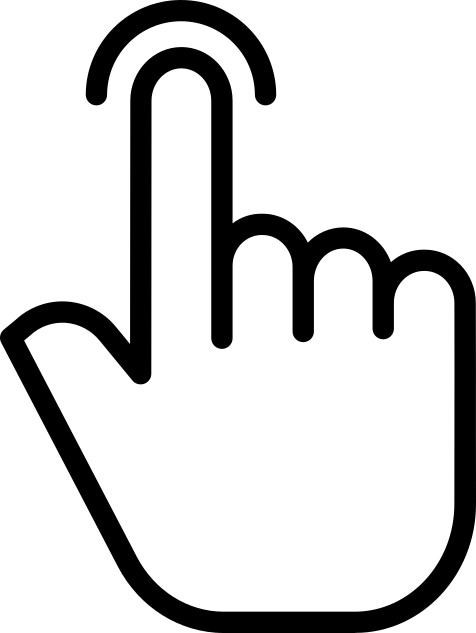
\includegraphics[width=0.03\textwidth]{static/dedo.png}} ;
         \node[factor, minimum size=1cm, xshift=3cm] (p3) {} ;
         
         \node[const, above=of p1, yshift=.15cm] (fp1) {$1/3$};
         \node[const, above=of p2, yshift=.15cm] (fp2) {$0$};
         \node[const, above=of p3, yshift=.15cm] (fp3) {$2/3$};
         \node[const, below=of p2, yshift=-.10cm, xshift=0.3cm] (dedo) {};
        } 
\end{figure}
  
Esta respuesta es diferente a la que obtuvimos con el primer modelo causal.
Sin embargo, ambas comparten la propiedad de ser la distribución de creencias que maximiza la incertidumbre dada la evidencia formal (modelo causal) y empírica (datos), lo que hace que sean proposiciones sobre las que podemos acordar tanto intercultural como intersubjetivamente.

\section{Teorema de Bayes}

\section{Selección de modelos}

\chapter{TrueSkill Through Time}

\chapter{Las implementaciones en Julia, Python y R}

\chapter{Efecto de los equipos sobre el aprendizaje (faithfull-sinergia)}

\chapter{Efecto de la topología sobre el aprendizaje.}

\chapter{Sistema de estimación para el juego Go (AAGo).}


\end{document}
